\section{Exploratory analysis}\label{sec:eda}

The descriptive statement was broken into twelve sub-questions. Before any table was computed, I recorded what I expected for each one. This section goes through them in order and ends with the correlation matrix.

\subsection*{How much free play is deducted? (sub-questions 1 and 2)}

Across the \V{fp_rows} months with a value, the median sportsbook-month deducted \$\V{fp_median} of free play for every \$100 wagered. Figure~\ref{fig:spread} shows one main bunch with a long tail: half of all months fall between \$\V{fp_q1} and \$\V{fp_q3}, while \V{fp_n_10plus} months (\V{fp_pct_10plus}\%) reach \$\V{def_fp_high} or more and the largest is \$\V{fp_max}. I expected two clusters. The only sign of a second group is \V{fp_n_under1} months (\V{fp_pct_under1}\%) under \$1.

\begin{figure}[H]
\centering
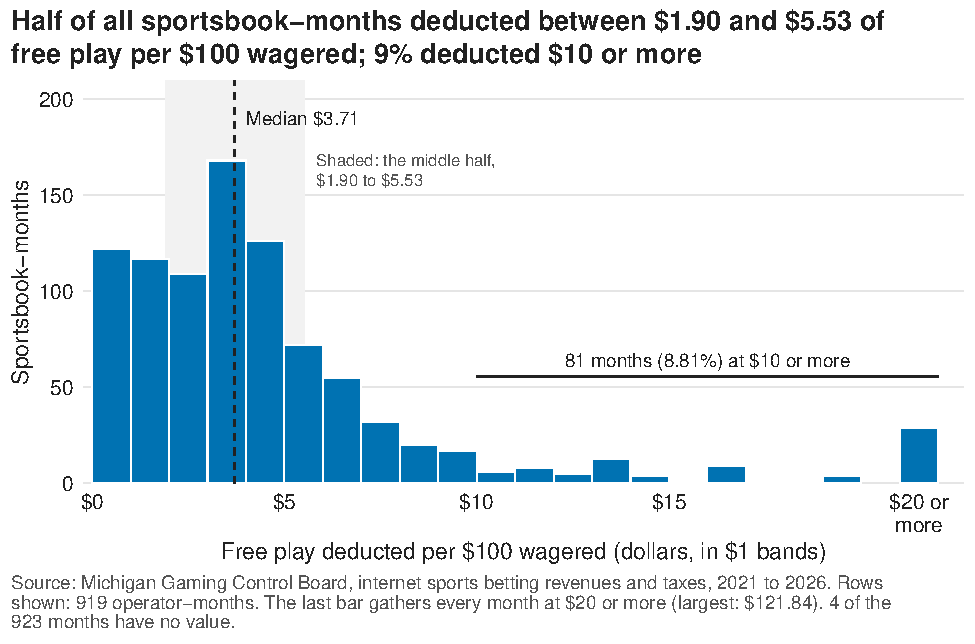
\includegraphics[width=0.92\linewidth]{figures/fig01_free_play_spread.pdf}
\caption{Spread of free play deducted per \$100 wagered (sub-question 1). Source: Michigan Gaming Control Board; \V{fp_rows} sportsbook-months.}\label{fig:spread}
\end{figure}

No state tax or payment was made in \V{notax_n} of the \V{rows_final} sportsbook-months (\V{notax_pct}\%), almost as many as the \V{tax_n} months (\V{tax_pct}\%) in which something was paid. Asked what I would have guessed before seeing any number, I said under 10\%.

\subsection*{Who are the sportsbooks, and which deduct the most? (sub-questions 3 and 4)}

The market is concentrated. Figure~\ref{fig:share} shows that three sportsbooks took \V{share_top3_total}\% of all dollars wagered: FanDuel (\V{share_top1}\%), DraftKings (\V{share_top2}\%) and BetMGM (\V{share_top3}\%). The nine smallest of the \V{n_operators} took \V{share_bottom9}\% together. I expected the top three to hold 50\% to 70\%.

\begin{figure}[H]
\centering
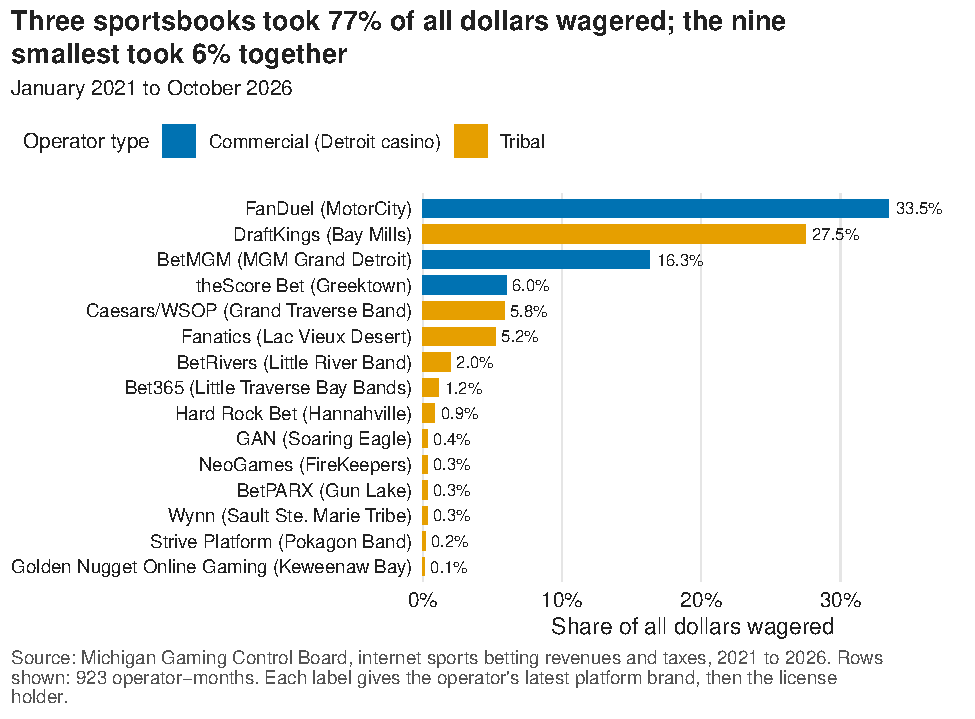
\includegraphics[width=0.92\linewidth]{figures/fig03_share_of_wagering.pdf}
\caption{Share of all dollars wagered by operator, colored by operator type (sub-question 3). Source: Michigan Gaming Control Board; \V{rows_final} sportsbook-months.}\label{fig:share}
\end{figure}

The biggest brands are not the heaviest users of free play per \$100. In Figure~\ref{fig:operators} the two highest medians belong to smaller tribal sportsbooks: Lac Vieux Desert (Fanatics) at \$\V{op_lvd_median} over \V{op_lvd_months} months and Hannahville (Hard Rock Bet) at \$\V{op_hannahville_median} over \V{op_hannahville_months}. BetMGM is third at \$\V{op_betmgm_median}. FanDuel (\$\V{op_fanduel_median}) and DraftKings (\$\V{op_draftkings_median}) sit beside the overall median of \$\V{fp_median}. The lowest median is Pokagon Band's \$\V{op_pokagon_median}, but its middle half runs from \$\V{op_pokagon_q1} to \$\V{op_pokagon_q3}, so a small sportsbook's months swing widely. I expected the big brands to deduct more. Table~\ref{tab:operators} gives the numbers behind both figures.

\begin{figure}[H]
\centering
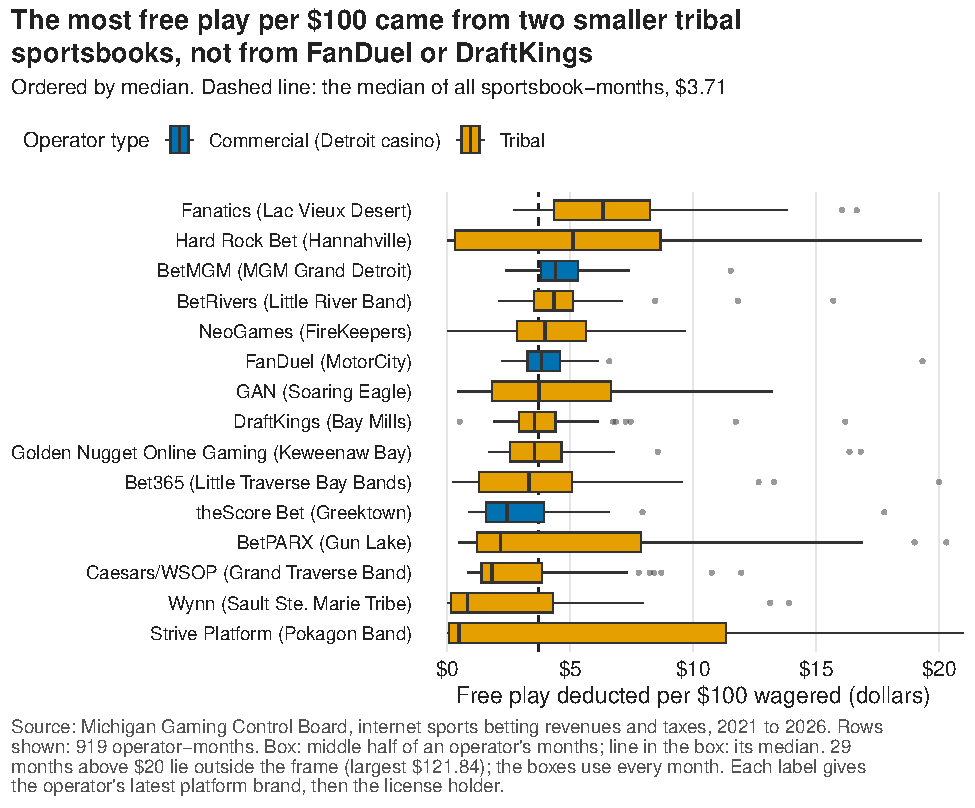
\includegraphics[width=0.92\linewidth]{figures/fig04_free_play_by_operator.pdf}
\caption{Free play deducted per \$100 wagered by operator, ordered by median (sub-question 4). \V{fp_n_20plus} months above \$\V{def_frame} are outside the frame. Source: Michigan Gaming Control Board; \V{fp_rows} sportsbook-months.}\label{fig:operators}
\end{figure}

\begin{table}[H]
\centering\footnotesize
\caption{Free play per \$100 wagered and share of all dollars wagered, by operator. Source: output/tables/eda\_03 and eda\_04.}\label{tab:operators}
% Written by scripts/08_report_numbers.R from output/tables. Do not edit by hand.
\begin{tabular}{@{}p{0.21\linewidth}p{0.20\linewidth}lrrrrr@{}}
\toprule
Operator & Brand & Type & Months & Lower quartile & Median & Upper quartile & Share of wagering (\%) \\
\midrule
Lac Vieux Desert & Fanatics & tribal & 70 & 4.34 & 6.34 & 8.25 & 5.23 \\
Hannahville & Hard Rock Bet & tribal & 66 & 0.31 & 5.13 & 8.67 & 0.87 \\
MGM Grand Detroit & BetMGM & commercial & 70 & 3.82 & 4.39 & 5.32 & 16.29 \\
Little River Band & BetRivers & tribal & 70 & 3.54 & 4.34 & 5.11 & 2.00 \\
FireKeepers & NeoGames & tribal & 64 & 2.83 & 3.96 & 5.63 & 0.34 \\
MotorCity & FanDuel & commercial & 70 & 3.26 & 3.83 & 4.57 & 33.48 \\
Soaring Eagle & GAN & tribal & 55 & 1.82 & 3.73 & 6.65 & 0.35 \\
Bay Mills & DraftKings & tribal & 70 & 2.91 & 3.54 & 4.39 & 27.46 \\
Keweenaw Bay & Golden Nugget Online Gaming & tribal & 37 & 2.54 & 3.54 & 4.64 & 0.13 \\
Little Traverse Bay Bands & Bet365 & tribal & 38 & 1.29 & 3.32 & 5.06 & 1.16 \\
Greektown & theScore Bet & commercial & 70 & 1.57 & 2.43 & 3.92 & 5.99 \\
Gun Lake & BetPARX & tribal & 63 & 1.20 & 2.16 & 7.87 & 0.33 \\
Grand Traverse Band & Caesars/WSOP & tribal & 70 & 1.39 & 1.82 & 3.84 & 5.85 \\
Sault Ste. Marie Tribe & Wynn & tribal & 39 & 0.14 & 0.83 & 4.30 & 0.32 \\
Pokagon Band & Strive Platform & tribal & 67 & 0.05 & 0.46 & 11.35 & 0.20 \\
\bottomrule
\end{tabular}

\end{table}

\subsection*{Is reliance on free play fading? (sub-questions 5, 6, 7 and 10)}

The yearly median fell from \$\V{yr_2021_median} per \$100 in 2021 (\V{yr_2021_months} months) to \$\V{yr_2023_median} in 2023 (\V{yr_2023_months}) and \$\V{yr_2026_median} in 2026 (\V{yr_2026_months}). Most of the drop came in the first two years. I expected it to rise.

Figure~\ref{fig:age} shows where the drop comes from. For tribal sportsbooks the median was \$\V{age_tri_b1_median} per \$100 in their first six months (\V{age_tri_b1_months} months), \$\V{age_tri_b2_median} in the next six (\V{age_tri_b2_months}), \$\V{age_tri_b3_median} in the second year (\V{age_tri_b3_months}) and \$\V{age_tri_b5_median} after four years (\V{age_tri_b5_months}). For the commercial sportsbooks it stayed between \$\V{age_com_min} and \$\V{age_com_max} at every age, although their first two age bands hold only \V{age_com_b1_months} months each, fewer than the \V{def_small_group} this report treats as a minimum. I expected free play to be high at launch and then drop fast, which holds for tribal sportsbooks and not for commercial ones.

\begin{figure}[H]
\centering
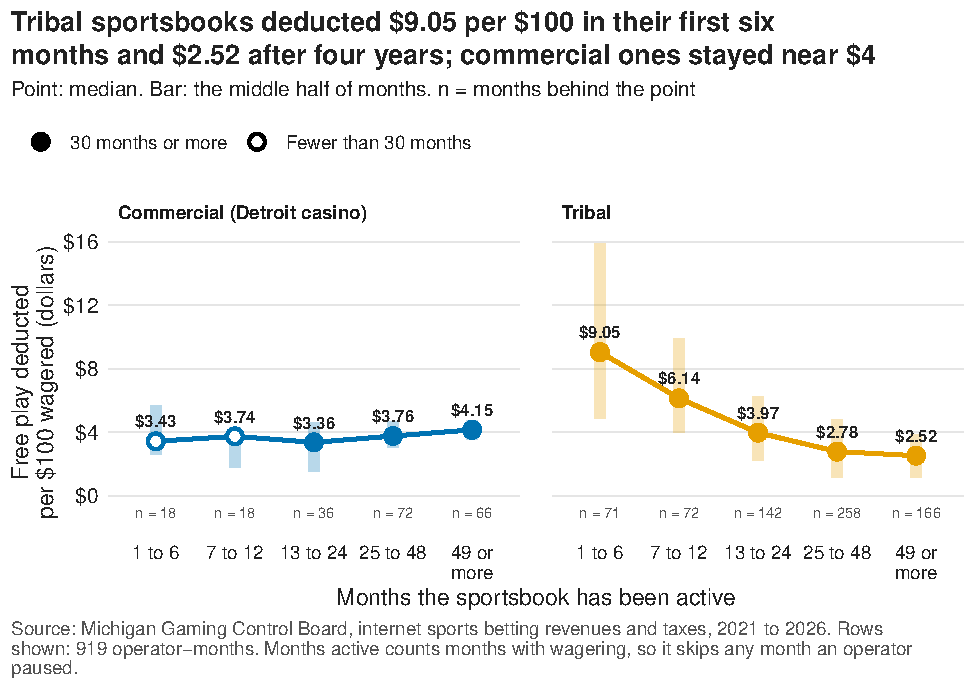
\includegraphics[width=0.92\linewidth]{figures/fig10_free_play_by_age_and_type.pdf}
\caption{Median free play per \$100 wagered by months active, within each operator type (sub-question 10). Source: Michigan Gaming Control Board; \V{fp_rows} sportsbook-months.}\label{fig:age}
\end{figure}

Taking all months together, the two operator types are close: a median of \$\V{com_median} for commercial sportsbooks (\V{com_months} months) and \$\V{tri_median} for tribal ones (\V{tri_months}). Tribal months are far more spread out, with a middle half from \$\V{tri_q1} to \$\V{tri_q3} against \$\V{com_q1} to \$\V{com_q3}. Size tells little: the correlation between free play per \$100 and the size of the month is \V{r_fp_size} across \V{fp_rows} months. Months under \$1 million wagered have the lowest median (\$\V{size_band1_median}, \V{size_band1_months} months) and the three larger size bands are nearly level (\$\V{size_band2_median}, \$\V{size_band3_median} and \$\V{size_band4_median}). I expected commercial sportsbooks and bigger months to show more free play.

\subsection*{How often is no tax paid, and by whom? (sub-questions 8 and 9)}

Tribal sportsbooks paid nothing to the State in \V{tri_notax_n} of \V{tri_rows} months (\V{tri_notax_pct}\%), commercial ones in \V{com_notax_n} of \V{com_rows} (\V{com_notax_pct}\%), as I expected. Figure~\ref{fig:notax} adds time. For tribal sportsbooks the share fell from \V{tri_2021_notax_pct}\% in 2021 (\V{tri_2021_notax_n} of \V{tri_2021_rows} months) to \V{tri_2026_notax_pct}\% in 2026 (\V{tri_2026_notax_n} of \V{tri_2026_rows}), with a bump back to \V{tri_2024_notax_pct}\% in 2024. For the commercial sportsbooks it swung: \V{com_2022_notax_round}\% in 2022, \V{com_2024_notax_pct}\% in 2024 (\V{com_2024_notax_n} of \V{com_2024_rows} months), \V{com_2025_notax_pct}\% in 2025 and \V{com_2026_notax_round}\% in 2026. The 2026 figures cover January to October. I expected the share to rise. Table~\ref{tab:notax} gives every count.

\begin{figure}[H]
\centering
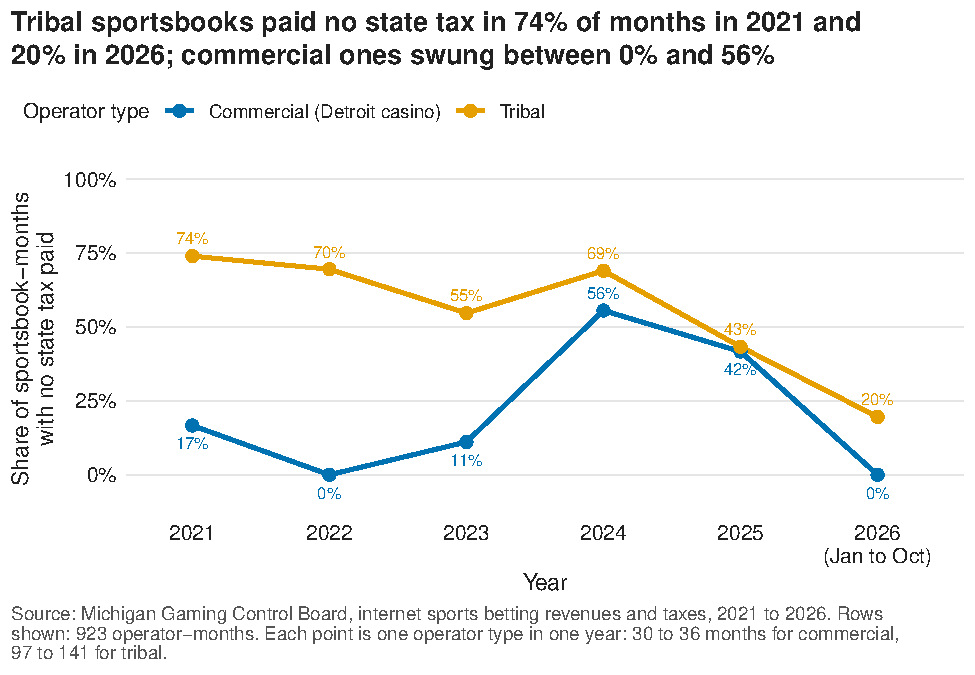
\includegraphics[width=0.92\linewidth]{figures/fig09_no_tax_by_year_and_type.pdf}
\caption{Share of sportsbook-months with no state tax paid, by year and operator type (sub-question 9). Source: Michigan Gaming Control Board; \V{rows_final} sportsbook-months.}\label{fig:notax}
\end{figure}

\begin{table}[H]
\centering\small
\caption{Months with no state tax paid, by year and operator type. Source: output/tables/eda\_09.}\label{tab:notax}
% Written by scripts/08_report_numbers.R from output/tables. Do not edit by hand.
\begin{tabular}{@{}llrrr@{}}
\toprule
Year & Operator type & Months & Months with no tax & Share with no tax (\%) \\
\midrule
2021 & commercial & 36 & 6 & 16.67 \\
2021 & tribal & 119 & 88 & 73.95 \\
2022 & commercial & 36 & 0 & 0.00 \\
2022 & tribal & 141 & 98 & 69.50 \\
2023 & commercial & 36 & 4 & 11.11 \\
2023 & tribal & 139 & 76 & 54.68 \\
2024 & commercial & 36 & 20 & 55.56 \\
2024 & tribal & 113 & 78 & 69.03 \\
2025 & commercial & 36 & 15 & 41.67 \\
2025 & tribal & 104 & 45 & 43.27 \\
2026 & commercial & 30 & 0 & 0.00 \\
2026 & tribal & 97 & 19 & 19.59 \\
\bottomrule
\end{tabular}

\end{table}

\subsection*{Do the unusual months change the picture? (sub-question 11)}

Leaving out the \V{lump_months} lump-deduction months and the \V{first_months} first months moves the overall median only from \$\V{fp_median} to \$\V{without_median} (\V{without_months} months left). Averages are another matter: the mean falls from \$\V{fp_mean} to \$\V{without_mean}, and the 2021 median from \$\V{yr_2021_median} to \$\V{without_2021}, because \V{lump_2021} of the lump months and \V{first_2021} of the first months fall in 2021. I expected no change at all. This report therefore uses medians, and the early-period numbers should be read with the flagged months in mind.

\subsection*{Which variables move together? (sub-question 12)}

Figure~\ref{fig:heatmap} is the correlation matrix of the two targets and the variables around them. Among things known before a month starts, free play per \$100 is most closely related to its own value the month before (\V{r_fp_prior}, \V{r_fp_prior_rows} months) and then to months active (\V{r_fp_months}). Paying no tax is most closely related to paying none the month before (\V{r_nt_prior}, \V{r_nt_prior_rows} months), to the size of the previous month (\V{r_nt_priorsize}) and to operator type (\V{r_nt_commercial} for commercial). My guess was that size would matter most for free play; its correlation is \V{r_fp_size}. Table~\ref{tab:corr} lists the correlations with each target.

The lump-deduction flag has the highest correlation with free play per \$100 of all (\V{r_fp_lump}), but it is built from the same month's deduction, so it is another version of the target and cannot be used to predict it. A correlation shows that two things move together in a straight line. It does not show that one causes the other.

\begin{figure}[H]
\centering
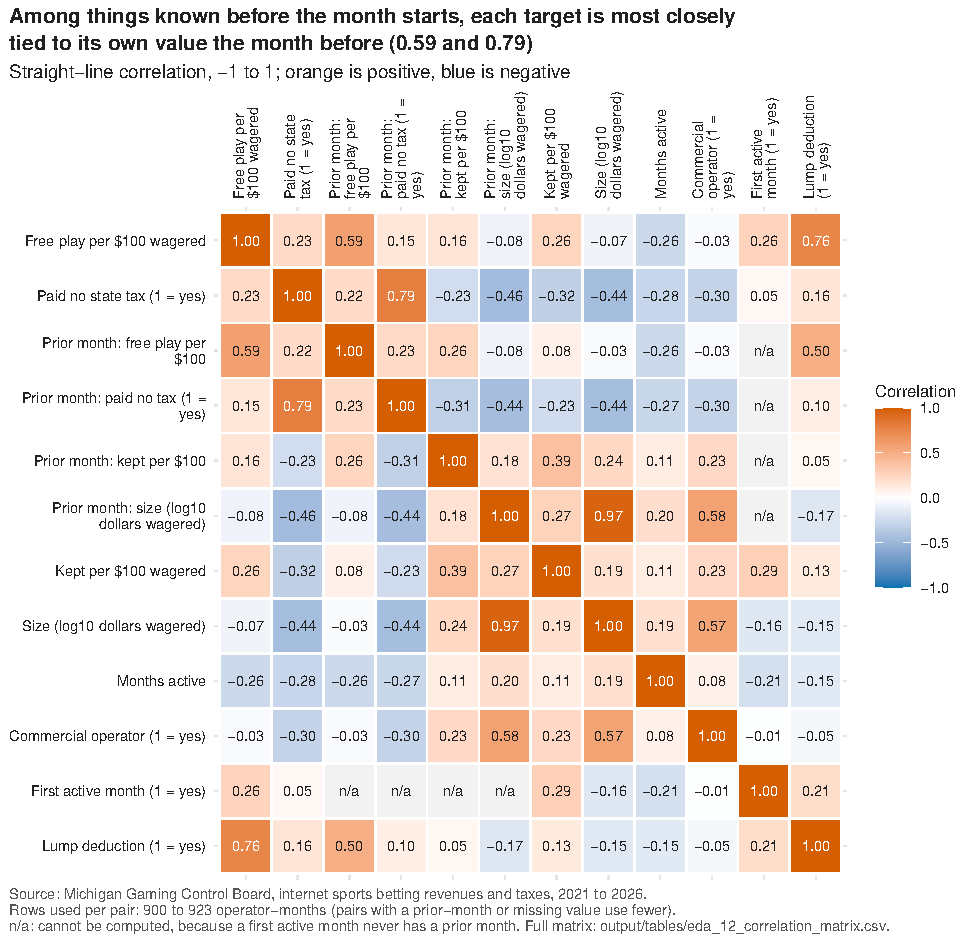
\includegraphics[width=\linewidth]{figures/fig12_correlation_heatmap.pdf}
\caption{Correlation matrix of the two targets and related variables (sub-question 12). Source: Michigan Gaming Control Board; \V{m1_rows} to \V{rows_final} sportsbook-months per pair.}\label{fig:heatmap}
\end{figure}

\begin{table}[H]
\centering\small
\caption{Correlation of each target with the variables known before the month starts. Source: output/tables/eda\_12c.}\label{tab:corr}
% Written by scripts/08_report_numbers.R from output/tables. Do not edit by hand.
\begin{tabular}{@{}p{0.27\linewidth}p{0.42\linewidth}rr@{}}
\toprule
Target & Variable known before the month starts & Correlation & Rows used \\
\midrule
Free play per \$100 wagered & Prior month: free play per \$100 & 0.59 & 900 \\
Free play per \$100 wagered & Months active & -0.26 & 919 \\
Free play per \$100 wagered & Year & -0.21 & 919 \\
Free play per \$100 wagered & Prior month: kept per \$100 & 0.16 & 902 \\
Free play per \$100 wagered & Prior month: paid no tax (1 = yes) & 0.15 & 903 \\
Free play per \$100 wagered & Prior month: size (log10 dollars wagered) & -0.08 & 903 \\
Free play per \$100 wagered & Month of the year (1 to 12) & -0.05 & 919 \\
Free play per \$100 wagered & Commercial operator (1 = yes) & -0.03 & 919 \\
Paid no state tax (1 = yes) & Prior month: paid no tax (1 = yes) & 0.79 & 906 \\
Paid no state tax (1 = yes) & Prior month: size (log10 dollars wagered) & -0.46 & 906 \\
Paid no state tax (1 = yes) & Commercial operator (1 = yes) & -0.30 & 923 \\
Paid no state tax (1 = yes) & Months active & -0.28 & 923 \\
Paid no state tax (1 = yes) & Prior month: kept per \$100 & -0.23 & 905 \\
Paid no state tax (1 = yes) & Year & -0.22 & 923 \\
Paid no state tax (1 = yes) & Prior month: free play per \$100 & 0.22 & 903 \\
Paid no state tax (1 = yes) & Month of the year (1 to 12) & -0.07 & 923 \\
\bottomrule
\end{tabular}

\end{table}
